\documentclass[journal,12pt,twocolumn]{IEEEtran}
\usepackage{cite}
\usepackage{amsmath,amssymb,amsfonts,amsthm}
\usepackage{algorithmic}
\usepackage{graphicx}
\usepackage{textcomp}
\usepackage{xcolor}
\usepackage{txfonts}
\usepackage{listings}
\usepackage{enumitem}
\usepackage{mathtools}
\usepackage{gensymb}
\usepackage{comment}
\usepackage[breaklinks=true]{hyperref}
\usepackage{tkz-euclide}
\usepackage{listings}
\usepackage{gvv}
\def\inputGnumericTable{}
\usepackage[latin1]{inputenc}
\usepackage{color}
\usepackage{array}
\usepackage{longtable}
\usepackage{calc}
\usepackage{multirow}
\usepackage{hhline}
\usepackage{ifthen}
\usepackage{lscape}

\newtheorem{theorem}{Theorem}[section]
\newtheorem{problem}{Problem}
\newtheorem{proposition}{Proposition}[section]
\newtheorem{lemma}{Lemma}[section]
\newtheorem{corollary}[theorem]{Corollary}
\newtheorem{example}{Example}[section]
\newtheorem{definition}[problem]{Definition}
\newcommand{\BEQA}{\begin{eqnarray}}
    \newcommand{\EEQA}{\end{eqnarray}}
\newcommand{\define}{\stackrel{\triangle}{=}}
\theoremstyle{remark}
\newtheorem{rem}{Remark}
\begin{document}
    
    \bibliographystyle{IEEEtran}
    \vspace{3cm}
    
    \title{Gate 2023 EE Q36}
    \author{EE23BTECH11212 - Manugunta Meghana Sai$^{*}$% <-this % stops a space
    }
    \maketitle
    \newpage
    \bigskip
    
    \renewcommand{\thefigure}{\theenumi}
    \renewcommand{\thetable}{\theenumi}
    
    \vspace{3cm}
    \textbf{Gate 2023 EE Q36} 
    The magnitude and phase plots of an LTI systems are shown in figure. Find the transfer function.\\
    \begin{figure}[h!]
        \centering
        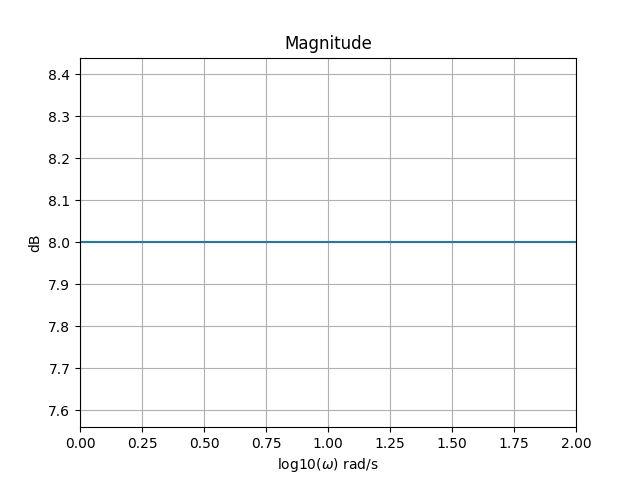
\includegraphics[width=\columnwidth]{figs/gain_plot.png}
        \caption{Magnitude}
        \label{fig:1ee36}
    \end{figure}
    
    \begin{figure}[h!]
        \centering
        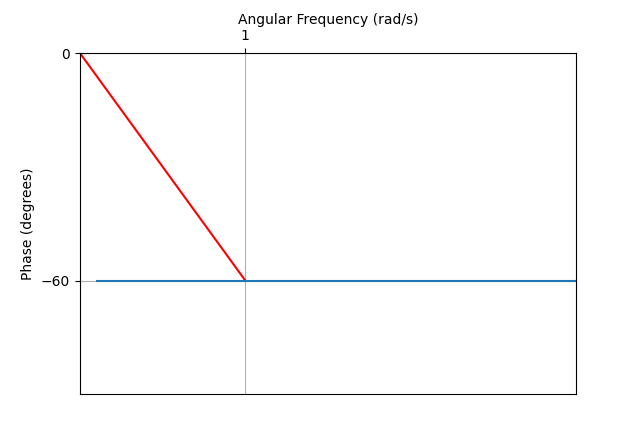
\includegraphics[width=\columnwidth]{figs/graph2.png}
        \caption{Phase}
        \label{fig:2ee36}
    \end{figure}
    
    \solution
    From the graph~\ref{fig:1ee36}, we can infer that the magnitude of the transfer function does not change with $\omega$.
    \begin{align}
        |\mathrm{H}(j\omega)|\, (\mathrm{dB}) &= 20\log_{10}(|\mathrm{H}(j\omega)|) \nonumber \\
        8 &= 20\log_{10}(|\mathrm{H}(j\omega)|) \nonumber \\
        |\mathrm{H}(j\omega)| &= 10^{0.4} = 2.511
    \end{align}
    From the graph~\ref{fig:2ee36}, we can infer the relation between phase and $\omega$:
    \begin{align}
        \text{phase} = \frac{-\pi}{3}\omega
    \end{align}
    The direction of the transfer function is:
    \begin{align}
        e^{-j\frac{\pi}{3}\omega}
    \end{align}
    The transfer function is a product of its magnitude and direction,
    \begin{align}
        H(j\omega) &= 2.511 e^{-j\frac{\pi}{3}\omega} \\
        &= 2.511 e^{-0.032s}
    \end{align}
    \setcounter{figure}{1} % Set figure counter to 1
\end{document}

